\documentclass[a4paper,11pt]{article}

\usepackage[utf8]{inputenx}
\usepackage[style=apa,backend=biber,alldates=edtf,maxcitenames=3]{biblatex}
\usepackage[nottoc,notlot,notlof]{tocbibind}
\usepackage[font={it}, labelfont=bf]{caption}
\usepackage{hyperref}
\usepackage[braket, qm]{qcircuit}
\usepackage{a4wide}
\usepackage{enumitem}
\usepackage{fancyhdr}
\usepackage{blochsphere}
\usepackage{xcolor}
\usepackage{amssymb}
\usepackage{amsmath}
\usepackage{subcaption}
\usepackage{multicol}
\usepackage{dirtytalk}
\usepackage{tikz-3dplot}
\usetikzlibrary{3d}

\DeclareFieldFormat[article,unpublished,misc,online]{title}{\textit{#1}}

\renewcommand{\abstractname}{Summary}

\renewcommand*{\arraystretch}{1.1}

\DeclareMathOperator{\sgn}{sgn}

\newcommand{\qstatezero}{
	\begin{pmatrix}1 \\ 0\end{pmatrix}
}
\newcommand{\qstateone}{
	\begin{pmatrix}0 \\ 1\end{pmatrix}
}

\newcommand{\hgate}{
	\dfrac{1}{\sqrt2}
	\begin{pmatrix}
		1 & \phantom{-}1 \\
		1 & -1
	\end{pmatrix}
}

\addbibresource{quantum-internship-research-paper.bib}

\title{Simulation of Quantum Algorithms for Solving Machine Learning and Chemistry Problems}
\author{Steven Oud (500776959) \\ \emph{SURFsara}}
\date{\today}

\begin{document}

\maketitle

\begin{abstract}
Lorem ipsum dolor sit amet, consectetur adipiscing elit. Fusce lobortis erat eget erat euismod dapibus. Interdum et malesuada fames ac ante ipsum primis in faucibus. Donec pharetra, magna ac tincidunt varius, neque odio lobortis velit, eget tincidunt lectus sapien ac velit. Donec maximus euismod arcu, at efficitur urna. Praesent viverra elementum elementum. Cras lacinia nisi eleifend sodales posuere. Fusce ut blandit purus, quis ornare est. Aenean varius purus lorem, a lobortis orci mollis pretium. Nulla facilisi. Nulla in neque orci. Integer dolor massa, ullamcorper nec sagittis id, mattis a lectus. Vivamus efficitur mi a elit feugiat facilisis. Ut lorem tortor, dignissim nec quam et, dapibus vehicula nibh. Quisque mollis enim quis odio interdum, ac blandit mauris maximus. Aenean ac dolor in augue accumsan porta.

Fusce at sodales turpis. Nullam pulvinar rhoncus diam eu consequat. Sed et ante ac augue rutrum cursus id id mi. Quisque aliquet at lectus eget condimentum. Quisque pharetra nulla vel vestibulum vulputate. Donec blandit lacus est, sed tempor nisi laoreet eget. Mauris maximus ultricies varius. Nullam id hendrerit ante, quis efficitur nibh. Pellentesque convallis dignissim dapibus. Nunc vehicula scelerisque posuere.
\end{abstract}

\newpage

\tableofcontents

\newpage

\section{Introduction}
Quantum computing is one of the most promising technology developments of the coming years.
Big companies like IBM (\cite{ibm-quantum}), Google (\cite{google-quantum}), Intel (\cite{intel-quantum}), Microsoft (\cite{microsoft-quantum}), and countries like the USA and China are investing huge amounts of money into the development and building of meaningful working quantum computers (\cite{usa-quantum, china-quantum}).
The development of practical quantum computers that can be used to solve real-world problems is driven by the expectation that for certain tasks, quantum computers can outperform classical computers (\cite{preskill-qc}).

Already last year, SURFsara started a number of activities and collaborations in the field of quantum computing.
The overall objective of SURFsara is to support Dutch researchers in taking an early and competitive advantage in quantum computing technologies and facilities while these become available.
Like with any  emerging compute technology, it needs early adopters in the scientific computing community to identify problems of practical interest that are suitable as proof-of-concept applications.
In the context of the SURF Open Innovation Lab, SURFsara seeks to stimulate and support these advances in scientific research in close collaboration with research groups.
Within this context SURFsara is interested in testing, benchmarking and creating good examples of quantum computing applications that can be used by the scientific community.

SURFsara HPC center supports various research institutes and universities of the Netherlands.
The chemistry community is currently one of the largest; the machine learning community is probably the fastest growing one.
Both of these fields are large areas of research within the quantum computing field, expecting large improvements to be gained from them.
As the main interest of SURFsara is to support the potential main use cases of quantum computers in the future, the tasks of this internship will be focused on quantum machine learning (QML) and quantum chemistry (QC) algorithms.
This internship aims to research state-of-the-art QML and QC algorithms, run simulations of them and benchmark them.

This report will try to give an answer to the main question ``\emph{How can quantum algorithms be implemented using simulated quantum circuits to solve machine learning and chemistry problems?}"
This is further expanded into the following sub questions:
\begin{enumerate}
	\item What are current promising QML and QC algorithms?
	\item What simulators are best suited for simulating QML and QC quantum circuits?
	\item How can these quantum algorithms be integrated in current classical workflow of chemistry and machine learning applications?
	\item How do these quantum algorithms perform (in regard to classical algorithms)?
\end{enumerate}

This report is structured as follows. First, in Section~\ref{sec:methods}, I describe how the research was conducted.
Second, in Section~\ref{sec:quantum-computation-information}, a short introduction to quantum computation and information is given.
Third, in Section~\ref{sec:quantum-ml} and Section~\ref{sec:quantum-chemistry}, research towards quantum machine learning and quantum chemistry is described.
Finally, in Section~\ref{sec:implementation-and-results}, quantum algorithms are implemented using simulation and the results are discussed.
The conclusion of the research is described in Section~\ref{sec:conclusion}.

\section{Methods} \label{sec:methods}
The research in this report was done mostly through desk research, with the help and advice of my colleagues.
The first step was to get familiar with the QML and QC fields; what background knowledge is required, what is the current state of research and what are the next steps?
To get started, several papers in promising areas of research were provided by my colleagues. 
From there, databases such as Google Scholar and arXiv were used to find further information about these areas.
Search terms used include \emph{quantum machine learning}, \emph{quantum neural network}, \emph{quantum support vector machine}, \emph{variational quantum eigensolver}, \emph{quantum phase estimation}, \emph{quantum perceptron}, \emph{quantum classifier}, \emph{quantum machine learning library}, \emph{quantum chemistry simulation} and \emph{hybrid quantum optimization}.

\section{Quantum Computation and Information} \label{sec:quantum-computation-information}
Quantum computers take advantage of quantum mechanical effects such as superposition and entanglement to solve certain problems faster than classical computers.
The idea of a quantum computer was first proposed by Richard Feynman for simulating physics (\cite{feynman-simulating}).
Since then the field has advanced a lot with algorithms such as Shor's algorithm for factoring integers (\cite{shor-factoring}) and Grover's search algorithm (\cite{grover-search}).
These quantum algorithms show efficient solutions for problems that are considered hard for classical computers.

This section summarizes basic concepts of quantum computation and information theory required to understand how quantum computers can be used to speedup certain computational problems.
This is a very high level overview of quantum computation and is far from a complete introduction to the field.
For a more complete introduction to quantum computation and information, refer to the book by~\cite{nielsen-chuang}.

\subsection{Quantum States}
The basic and smallest unit of quantum information is the quantum bit, or \emph{qubit}.
A qubit is a two-state quantum-mechanical system, which can be represented for example in the spin of an electron.
A qubit can be in a state of an orthonormal basis $\{\ket{0}, \ket{1}\}$ (corresponding to spin up and spin down for the electron example), but it can also be in a linear combination, or \emph{superposition}, of states.
The state of a qubit (the so-called \emph{wave function}) can be described as following:
\begin{equation}
\ket{\psi} = c_0\ket{0} + c_1\ket{1}.
\end{equation}
Quantum states are denoted using Dirac notation \ket{\cdotp}, which is a column vector in $\mathbb{C}^n$.
Here the coefficients $\{c_0, c_1\}$ are complex valued numbers called \emph{probability amplitudes}.
When we measure a quantum state, it collapses probabilistically to one of the basis states.
The norm square $|c_0|^2$ gives us the probability of finding the particle in state \ket{0}, and $|c_1|^2$ gives us the probability of finding the particle in state \ket{1}.
As we are dealing with probabilities, the quantum state should be normalized: $\sum_{i=0}|c_i|^2 = 1$.
As an example we have the arbitrary state:
\begin{equation}
\ket{\psi} = \dfrac{i}{2}\ket{0} - \dfrac{\sqrt3}{2}\ket{1}.
\end{equation}
After measuring this state, we have a $|i/2|^2 = 1/4$ chance of the system being in the state \ket{0}, and a $|-\sqrt3/2|^2 = 3/4$ chance of being in the state \ket{1}.
Note that we cannot observe the amplitudes of a quantum state.
When we measure a state, it collapses to a basis state \ket{j} with probability $|c_j|^2$.
If we measure again immediately after the first measure, we get the same result 100\% of the time.
So if we measure \ket{1} and measure again immediately after, we will see \ket{1} again.
Measuring a quantum state collapses the wave function and destroys state information.

We define the computational basis states $\{\ket{0}, \ket{1}\}$ as following:
\begin{equation}
\ket{0} = \qstatezero{}, \quad
\ket{1} = \qstateone{}.
\end{equation}
This idea generalizes to multi-qubit systems.
A multi-qubit system with $n$ states $\{\ket{\psi_1}, \ket{\psi_2}, \ldots, \ket{\psi_n}\}$ can be represented using the \emph{Kronecker product}\footnote{Entangled states are an exception to this, which will be further discussed in Section~\ref{sec:entanglement}}:
\begin{equation}
\ket{\psi} = \ket{\psi_1} \otimes \ket{\psi_2} \otimes \dotsm \otimes \ket{\psi_n},
\end{equation}
resulting in a $N = 2^n$ dimensional state \ket{\psi}.
For example, a three qubit state lives in a  $2^3$-dimensional Hilbert space spanned by computational basis states $\{\ket{000}, \ket{001}, \ket{010}, \ldots, \ket{111}\}$:
\begin{equation}
\begin{aligned}
\ket{\psi} &= c_0\ket{000} + c_1\ket{001} + c_2\ket{010} + \dotsm + c_{N-1}\ket{111} \\
&= c_0\begin{pmatrix}1 \\ 0 \\ 0 \\ \vdots \\ 0\end{pmatrix} + c_1\begin{pmatrix}0 \\ 1 \\ 0 \\ \vdots \\ 0\end{pmatrix} + c_2\begin{pmatrix}0 \\ 0 \\ 1 \\ \vdots \\ 0\end{pmatrix} + \dotsm + c_{N-1}\begin{pmatrix}0 \\ 0 \\ 0 \\ \vdots \\ 1\end{pmatrix} = \begin{pmatrix}c_0 \\ c_1 \\ c_2 \\ \vdots \\ c_{N-1}\end{pmatrix}.
\end{aligned}
\end{equation}

\subsection{Quantum State Evolution}
In classical computers, we manipulate bits through logical gates.
Quantum computers use quantum gates, which transforms one quantum state to another through an operator $U$.
These operators must be unitary.
That is, they must preserve the norm of the vector and be reversible: $U^\dagger U = UU^\dagger = I$ (where $^\dagger$ is the complex conjugate and $I$ the identity matrix).
Single qubit states can be thought of as a vector on the surface of a sphere (the Bloch sphere).
A unitary operation can then be thought of as rotations around the $x$, $y$ and $z$ axes of the sphere (Figure~\ref{fig:bloch-sphere}).

\begin{figure}[ht]
	\centering
	\hspace{1.175cm}
	\begin{blochsphere}[radius=1.75cm, tilt=15, rotation=-20, opacity=0.1, color=white]
		\drawBallGrid[style={opacity=0.1}]{30}{30}
		
		\drawStatePolar[axisarrow=true, statewidth=0.5]{x-axis}{90}{90}
		\drawStatePolar[axisarrow=true, statewidth=0.5]{y-axis}{90}{0}
		\drawStatePolar[axisarrow=true, statewidth=0.5]{z-axis}{0}{0}
		\node[left] at (x-axis) {$x$};
		\node[right] at (y-axis) {$y$};
		\node[left] at (z-axis) {$z$};
		
	    \drawBallGrid[style={opacity=0.25, loosely dashed}]{180}{180}
		
		\drawStatePolar[statecolor=blue, statewidth=0.5, labelmark=true]{start_state}{15}{14}
		\node[above right] at (start_state) {\ket{\psi}};
		
		\drawStatePolar[statecolor=red, statewidth=0.5, labelmark=true]{end_state}{125}{14}
		\node[right=1mm] at (end_state) {$\ket{\psi'} = U\ket{\psi}$};
		
		\labelLatLon{up}{90}{0};
		\labelLatLon{down}{-90}{90};
		\node[above=1mm] at (up) {{\large \ket{0}}};
		\node[below=1mm] at (down) {{\large \ket{1}}};
	\end{blochsphere}
	\caption{Arbitrary transformation of state \ket{\psi} by operator $U$ visualized on the Bloch sphere.}
	\label{fig:bloch-sphere}
\end{figure}

As an example, the $X$ gate is equivalent to the classical \textsc{not}: $X\ket{0} = \ket{1}$ and $X\ket{1} = \ket{0}$.
It is known as one of the three Pauli matrices used in quantum mechanics:
\begin{equation}
\sigma_1 = \sigma_x =
\begin{pmatrix}
0 & 1 \\
1 & 0
\end{pmatrix},
\quad
\sigma_2 = \sigma_y =
\begin{pmatrix}
0 & -i \\
i & \phantom{-}0
\end{pmatrix},
\quad
\sigma_3 = \sigma_z =
\begin{pmatrix}
1 & \phantom{-}0 \\
0 & -1
\end{pmatrix}.
\end{equation}
Another frequently used gate is the Hadamard gate, which produces an equal superposition:
\begin{equation}
H = \hgate{}.
\end{equation}
Which acts on the computational basis states as following:
\begin{equation}
\begin{aligned}
H\ket{0} &=
\hgate{}
\qstatezero{}
=
\dfrac{1}{\sqrt2}
\begin{pmatrix}1 \\ 1\end{pmatrix} \\
&= \dfrac{1}{\sqrt2}(\ket{0} + \ket{1}), \\
H\ket{1} &=
\hgate{}
\qstateone{}
=
\dfrac{1}{\sqrt2}
\begin{pmatrix}\phantom{-}1 \\ -1\end{pmatrix} \\
&= \dfrac{1}{\sqrt2}(\ket{0} + \ket{1}).
\end{aligned}
\end{equation}
Applying the Hadamard gate again on the equal superposition created above is an example of destructive interference:
\begin{equation}
\begin{aligned}
H\dfrac{1}{\sqrt2}(\ket{0} + \ket{1}) &= \ket{0}, \\
H\dfrac{1}{\sqrt2}(\ket{0} - \ket{1}) &= \ket{1}.
\end{aligned}
\end{equation}
We find that applying the Hadamard twice is the same as doing nothing, or more formally, we say the Hadamard gate is \emph{Hermitian}: $H = H^\dagger$.

\subsection{Entanglement} \label{sec:entanglement}
There also exist multi-qubit gates, which are required for universal quantum computing.
These gates introduce the phenomena entanglement.
Consider the following state:
\begin{equation}
\ket{\Phi^+} = \dfrac{1}{\sqrt2}(\ket{00} + \ket{11}).
\end{equation}
Measuring the first qubit gives state \ket{0} with probability $1/2$, and state \ket{1} with probability $1/2$.
However, the measurement immediately collapsed the whole state to either \ket{00} or \ket{11}.
So by measuring the first qubit, we also know the state of the second qubit.
The individual states are related to each other, and this relation is called entanglement.
More formally, two qubits are entangled if and only if the state of those two qubits cannot be expressed as two individual states.
For the entangled state \ket{\Phi^+}, let's assume there exist amplitudes $\{c_0,c_1,c'_0, c'_1\}$ such that:
\begin{equation}
\ket{\Phi^+} = (c_0\ket{0} + c_1\ket{1}) \otimes (c'_0\ket{0} + c'_1\ket{1}) = \dfrac{1}{\sqrt2}(\ket{00} + \ket{11}).
\end{equation}
However, this would imply that $c_0c'_0 = c_1c'_1 = 1/\sqrt2$ and $c_0c'_1 = c_1c'_0 = 0$, which does not have a solution.

The remarkable thing about entanglement is that it works over any distance.
That is, given the state \ket{\Phi^+}, one qubit could be located in another galaxy while the other qubit is located on earth.
When we measure the qubit on earth, we know that the qubit in the other galaxy is in the same state as we measured.
This does not allow for faster than light communication, as a classical channel is still required to communicate results between the observers.

\subsection{Quantum Speedup}
Quantum algorithms promise to provide a speedup over classical algorithms by ``abusing" quantum phenomena such as superposition, interference, exponential state space and entanglement.
They usually offer a quadratic or exponential speedup over their classical counterpart.
\cite{scott-aaronson-qc} probably described it best:
\say{The goal in quantum computing is to choreograph a computation so that the amplitudes leading to wrong answers cancel each other out, while the amplitudes leading to right answers reinforce.}

The most famous example of a quantum speedup is probably Shor's algorithm for factoring integers and computing discrete logarithms, which was introduced in 1994.
Its implications are huge for modern cryptography algorithms such as RSA, which depend on the fact that factoring integers is a hard problem on classical computers.
Shor showed that this can be done in polynomial time on a quantum computer~(\cite{shor-factoring}), providing an exponential speedup over classical algorithms. 
It has been estimated that a 2048-bit RSA integer could be factored in eight hours using 20 million noisy qubits (\cite{shor-20mil}).

\subsection{Current State of Quantum Computing}
It is important to note that quantum computers are still at the experimental stage, and a lot of results are theoretical.
For example, the highest number factored by using Shor's algorithm on an actual quantum computer thus far is 21~(\cite{shor-21}).
Furthermore, quantum supremacy, which is the potential ability of a quantum computer to solve problems that classical computers practically cannot~(\cite{preskill-qc}), has not been achieved yet as of writing this.
Current and near future quantum computers, often referred to as Noisy Intermediate-Scale Quantum (NISQ) devices, will have about 50-100 qubits and may be able to achieve quantum supremacy~(\cite{preskill-nisq}).
However, they suffer from noise, which greatly limits their coherence time and thus usefulness.
Quantum error correcting codes exist which can be used to protect from noise, but these require a high amount of qubits per logical qubit.

Research has adapted to the limitations of NISQ devices, and hybrid quantum/classical algorithms have become an important area of research.
Examples of such algorithms are the quantum approximate optimization algorithm (QAOA) for optimization problems~(\cite{qaoa}), and the variational quantum eigensolver (VQE) for finding eigenvalues of a Hamiltonian~(\cite{vqe}).
These hybrid algorithms typically involve a small quantum subroutine run inside of a classical optimization loop, removing the need for a large-scale, coherent quantum computer.

This research is focused on universal gate model quantum computers.
There exist special purpose quantum computers called quantum annealers, which have achieved qubit counts up to 2000~(\cite{dwave-2000}).
These quantum annealers are restricted to solving optimization problems, of which its usefulness has been doubted~(\cite{how-quantum-dwave, aaronson-dwave, detecting-quantum-speedup}).

\section{Quantum Machine Learning} \label{sec:quantum-ml}
Quantum machine learning is still in its early days of development, and lacks a widely recognized definition.
However, there have been promising developments in the recent years.

\section{Quantum Chemistry} \label{sec:quantum-chemistry}

\section{Implementation and Results} \label{sec:implementation-and-results}

\subsection{Quantum Neural Network}
A quantum neural network inspired by the work of~\cite{qnn-near-term} was implemented for classifying handwritten images.
The famous MNIST database of handwritten digits~(\cite{mnist-digits}) was used for this (Figure~\ref{fig:mnist}).
For initial experiment, the images of the data set were downsampled to a lower dimension and limited to binary classification of digits 1 and 8 to simplify the problem and reduce resource requirements.
After a successful initial experiment, the experiment is extended to multi-class classification of the original $28 \times 28$ data set.
\begin{figure}[ht]
	\centering
	\begin{subfigure}{.5\textwidth}
		\centering
		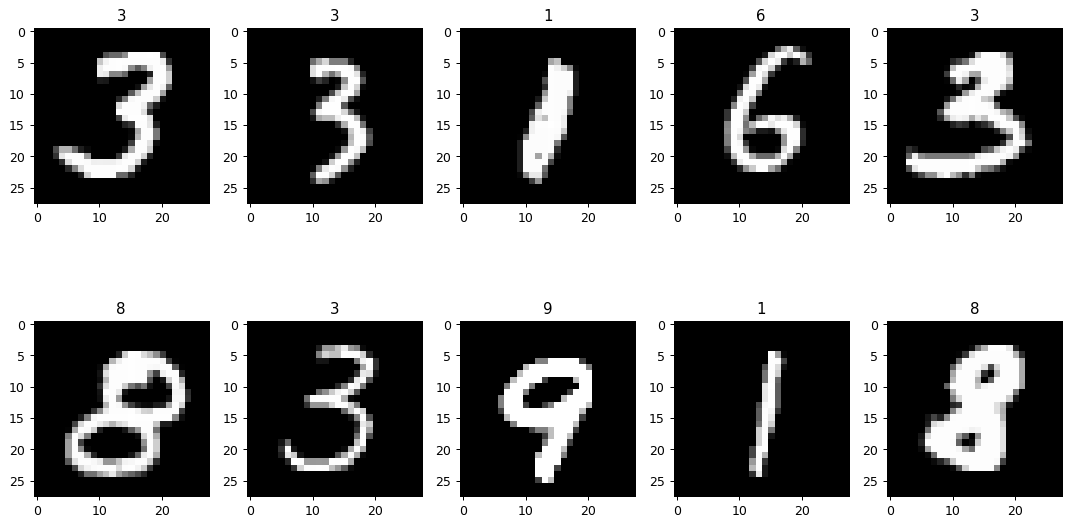
\includegraphics[width=.85\linewidth]{figures/mnist_28x28.png}
		\caption{Original data set of $28 \times 28$ images.}
		\label{fig:mnist_28x28}
	\end{subfigure}%
	\begin{subfigure}{.5\textwidth}
		\centering
		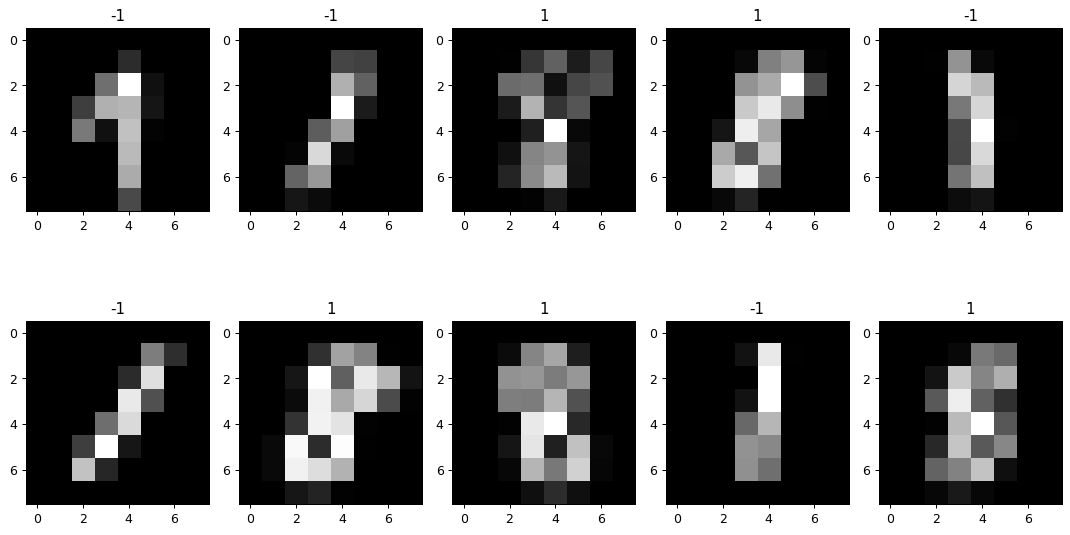
\includegraphics[width=.85\linewidth]{figures/mnist_8x8}
		\caption{Downsampled binary data set of $8 \times 8$ images.}
		\label{fig:mnist_8x8}
	\end{subfigure}
	\caption{Samples of MNIST data set used for quantum neural network binary classification.}
	\label{fig:mnist}
\end{figure}

\subsubsection{Binary Downsampled Classifier}
The problem of supervised classification in machine learning is defined as following: given a training set of data whose category is known, train a model which is able to identify to which category new data belongs.
A simple example that we will tackle in this section is recognizing if a handwritten digit is a 1 or an 8.

We implement a quantum neural network to classify $8 \times 8$ images of handwritten digits (Figure~\ref{fig:mnist_8x8}).
It uses a quantum circuit together with a classical optimization algorithm to find the optimal parameters for the quantum circuit, often known as a variational algorithm.
An overview of the quantum circuit used in the experiment can be found in Figure~\ref{fig:bdc-circuit}.
The variational quantum neural network works as following:
\begin{enumerate}
	\item Prepare data sample $\vec{x}$ in the amplitudes of a quantum state \ket{x} using for example qRAM~(\cite{qram}).
	\item Prepare a readout qubit in the state \ket{1}, giving \ket{x, 1}.
	\item Apply $L$ layers of parameterized unitaries: $U(\vec{\theta}_L) U(\vec{\theta}_{L-1}) \ldots U(\vec{\theta}_1)\ket{x, 1}$.
	\item Measure expectation value $\expval{Z}$ of readout qubit.
	\item Calculate and minimize the loss $L(\vec{\theta}, \expval{Z})$ through classical optimization algorithm.
	\item Repeat until converges.
\end{enumerate}
\begin{figure}[ht]
	\[
	\Large
	\Qcircuit @C=1em @R=0.3em @!R {
		& & \multigate{5}{U(\vec{\theta}_1)} & \multigate{5}{U(\vec{\theta}_2)} & \qw & & \multigate{5}{U(\vec{\theta}_L)} & \qw & \qw \\
		& & \ghost{U(\vec{\theta}_1)} & \ghost{U(\vec{\theta}_2)} & \qw & & \ghost{U(\vec{\theta}_L)} & \qw & \qw \\
		\lstick{\ket{x}~~} & & \ghost{U(\vec{\theta}_1)} & \ghost{U(\vec{\theta}_2)} & \qw & & \ghost{U(\vec{\theta}_L)} & \qw & \qw \\
		& ~~\vdots & & & ~~\hdots & & & \vdots \\
		& & \ghost{U(\vec{\theta}_1)} & \ghost{U(\vec{\theta}_2)} & \qw & & \ghost{U(\vec{\theta}_L)} & \qw & \qw \\
		& \lstick{\ket{1}} & \ghost{U(\vec{\theta}_1)} & \ghost{U(\vec{\theta}_2)} & \qw & & \ghost{U(\vec{\theta}_L)} & \meter & \rstick{\expval{Z}} \cw
		\gategroup{1}{1}{5}{1}{.7em}{\{}
	}
	\]
	\caption{General circuit of the quantum neural network classifier. The network consist of $L$ layers with each layer implementing a parameterized unitary $U(\vec{\theta}_i)$ whose parameters are optimized using a classical optimization algorithm. At the end of the circuit, the expectation value $\expval{Z}$ of the readout qubit is measured and the predicted class is decided by $\sgn(\expval{Z})$.}
	\label{fig:bdc-circuit}
\end{figure}

We trained a quantum neural network using a training set of 2014 images and a test set of 843 images.
As optimizer, we used the stochastic mini-batch gradient descent with a learning rate of $0.4$ and a batch size of $32$.
After training for 20 epochs, it managed to reach 91.1\% accuracy (Figure~\ref{fig:bdc-performance}) without any hyperparameter tuning or circuit optimization.
The goal of this experiment is not to compete with classical state-of-the-art neural networks, which are capable of achieving an error percentage of only 0.23\%~(\cite{cirecsan2012multi}).
Rather, it is meant to demonstrate the possibility of using quantum computers for machine learning problems.
It shows the potential, given we solve the issues surrounding qRAM (\cite{aaronson2015read}), to exploit the exponential growth of quantum state spaces to do machine learning on big data.
Quantum neural networks could also be used for learning about quantum data.
\begin{figure}[ht]
	\centering
	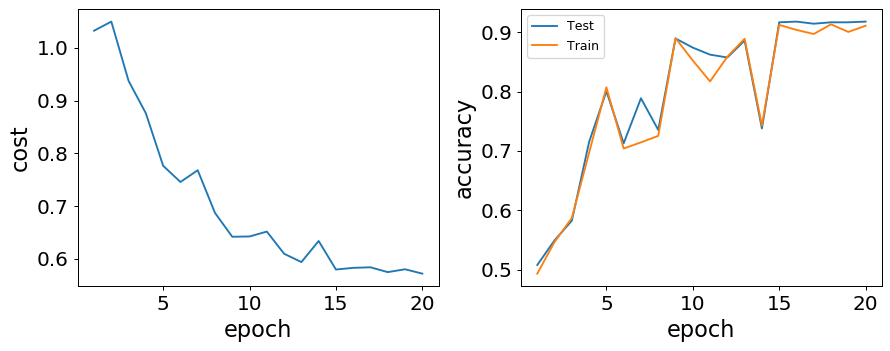
\includegraphics[width=.9\linewidth]{figures/downsampled_qnn.png}
	\caption{Quantum neural network performance on binary classification.}
	\label{fig:bdc-performance}
\end{figure}

\section{Conclusion} \label{sec:conclusion}

\printbibliography[heading=bibintoc]

\end{document}